%!TEX ROOT=formularioFisica.tex

\section{Elettromagnetismo}
Il padre di questa branca della fisica è Maxwell e con le sue quattro equazioni descrive il campo
elettro-magnetico e riassume le precedenti teorie.
\subsection{Le equazioni di Maxwell}
\begin{alignat*}{2}
  \Phi_{S_{ch}}(\vec{E},t) &= \frac{\sum q_i}{\varepsilon_0} &\quad \Phi_{S_{ch}}(\vec{B},t)&=0\\
  C_\Gamma(\vec{E},t) &= -\frac{\Delta \Phi(\vec{B})}{\Delta t} & C_\Gamma(\vec{B},t) &=
  \mu_0 \left[ i+\varepsilon_0 \frac{\Delta\Phi(\vec{E})}{\Delta t} \right]
\end{alignat*}
Queste sono le equazioni viste come funzione, anche se più spesso vengono definite attraverso
integrali
\begin{alignat*}{2}
  \int_{S_{ch}}\vec{E}\cdot\dif\vec{S} &= \frac{\sum q_i}{\varepsilon_0} &\quad 
  \int_{S_{ch}}\vec{B}\cdot\dif\vec{S}&=0\\
  \oint_\Gamma\vec{E}\cdot\dif\vec{l}&=-\der{\Phi(\vec{B})}{t} & 
  \oint_\Gamma\vec{B}\cdot\dif\vec{l}&=
  \mu_0 \left[ i+\varepsilon_0 \der{\Phi(\vec{E})}{t} \right]
\end{alignat*}
Le prime due leggi erano già presenti nei campi statici.

\subsection{La Terza legge di Maxwell}
La terza legge di Maxwell deriva dalla forza elettromotrice indotta. Se Faraday
ha trovato una forza elettromotrice indotta che produce la corrente, Maxwell va ancora più indietro
e l'unica cosa che può genera una forza elettromotrice è un \textbf{campo elettrico}.\\
Per andare a ricavare il campo elettrico, bisogna andare a ridefinire la forza
elettromotrice. Essa è il lavoro necessario a portare
l'unità di carica da un polo all'altro, diviso la carica. Quindi
\begin{equation*}
  \mathcal{E} = \frac{L_{+\to-}}{q}
\end{equation*}
Il lavoro però è definito come
\begin{equation*}
  \sum\limits^{n}_{i=1} \vec{F}\cdot\Delta\vec{l}_i = 
  \sum\limits^{n}_{i=1} \Delta q\vec{E}_i\cdot\vec{l}_i=
  \Delta q \sum\limits^{n}_{i=1} \vec{E}_i\cdot\vec{l}_i
\end{equation*}
Quindi ora possiamo riscrivere 
\begin{equation*}
  \mathcal{E}=\frac{\cancel{\Delta q}\sum\limits^{n}_{i=1}\vec{E}_i\cdot\vec{l}_i}{\cancel{\Delta q}}
  = C_\Gamma(\vec{E})
\end{equation*}
Ma se ora torniamo indietro, riscriviamo che
\begin{equation*}
  C_\Gamma(\vec{E}) = -\der{\Phi(\vec{B})}{t}
\end{equation*}
Nella definizione abbiamo utilizzato una somma. In realtà sarebbe il limite di una somma che quindi
definisce un integrale definito. Si riscrive generalmente
\begin{equation*}
  \oint_\Gamma\vec{E}\cdot\dif\vec{l} = -\der{\Phi(\vec{B})}{t}
\end{equation*}
Ed ecco la terza legge di Maxwell. Cosa ci dice però? Ci dice che se è presente una variazione di
flusso, si genera un campo elettrico perpendicolare a quello magnetico.
Immaginando una spira in un campo magnetico uniforme d'intensità variabile, immobile, la forza che 
agisce su di essa è
\begin{equation*}
  \vec{F} = q\vec{E}+q\vec{v}\times\vec{B}
\end{equation*}
ma essendo $\vec{v} = \vec{0}$ e quindi $q\vec{v}\times\vec{B} = 0$, dunque la forza che fa muovere
le cariche è pari a $q\cdot E_{ind}$. Se l'intensità di $\vec{B}$ varia, le linee di forza di 
$\vec{E}$ sono orientate in modo definito dalla legge di Lenz.

\subsection{La Quarta legge di Maxwell}
La quarta legge parte dall studio di un circuito RC in continua. Maxwell è andato a guardare la 
circuitazione tra le armature del condensatore.
La circuitazione calcolata prima dell'armatura è pari a
\begin{equation*}
  C_{\mathcolor{blue}{\Gamma_1}}(\vec{B}) = \mu_0\cdot i
\end{equation*}
dove $\mathcolor{blue}{\Gamma_1}$ è una linea chiusa attorno al filo conduttore. Se ora invece si 
prende una linea  $\mathcolor{red}{\Gamma_2}$ che passi attraverso le armature, la circuitazione sarà
\begin{equation*}
  C_{\mathcolor{red}{\Gamma_2}}(\vec{B}) = 0
\end{equation*}
in quanto non c'è corrente all'interno.
\begin{center}
  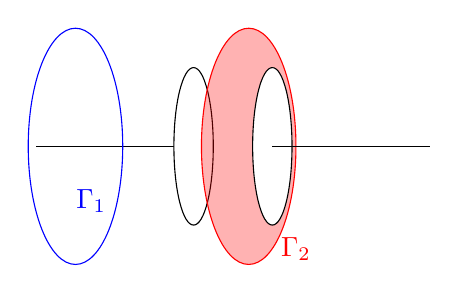
\begin{tikzpicture}
    \draw (0,0) -- (2,0);
    \draw[blue] (0.5,0) ellipse (0.6 and 1.5);
    \node[blue] at (0.7,-0.7) {$\Gamma_1$};
    \node[red] at (3.3,-1.3) {$\Gamma_2$};
    \filldraw[white,draw=black] (2,0) ellipse (0.25 and 1);
    \filldraw[fill opacity=0.3,red] (2.7,0) ellipse (0.6 and 1.5); 
    \filldraw[white,draw=black] (3,0) ellipse (0.25 and 1);
    \draw (3,0) -- (5,0);
  \end{tikzpicture}
\end{center}
Come si può capire però le due circuitazioni devono essere uguali. Maxwell per spiegare questo 
fenomeno, calcola il flusso del
campo elettrico su di una superficie $S$ circolare che ha come contorno la linea 
$\mathcolor{red}{\Gamma_2}$ possiamo calcolare semplicemente il flusso
\begin{equation*}
  \Delta\Phi(\vec{E}) = S \left[ \vec{E}(t+\Delta t)-\vec{E}(t) \right]
\end{equation*}
Sapendo che in un condensatore
\begin{equation*}
  E = \frac{\sigma}{\varepsilon_0} = \frac{q}{\varepsilon_0 S}
\end{equation*}
All'istante $t$, abbiamo una carica $q(t)$. All'istante $t+\Delta t$ invece abbiamo carica 
$q(t+\Delta t)$. Ma come possiamo riscriverla? Sapendo che
\begin{equation*}
  \Delta q = i\Delta t
\end{equation*}
e quindi 
\begin{equation*}
  q(t+\Delta t) = q(t) + i\Delta t
\end{equation*}
Avendo queste informazioni possiamo sostituirle nella formula del flusso di prima
\begin{equation*}
  \Delta\Phi(\vec{E})= \left[ \frac{q+i\Delta t}{\varepsilon_0 S}-\frac{q}{\varepsilon_0 S} \right]
\end{equation*}
Semplificando otteniamo
\begin{equation*}
  \Delta\Phi(\vec{E}) = \frac{i\Delta t}{\varepsilon_0}
\end{equation*}
Abbiamo così trovato il termine mancante, una corrente mai rilevata prima.
\begin{equation*}
  i_s = \varepsilon_0\frac{\Delta\Phi(\vec{E})}{\Delta t}
\end{equation*}
Questa è definita \textbf{corrente di spostamento}.\\
Tornando al problema originale, la circuitazione diventa quindi
\begin{equation*}
  \oint_\Gamma \vec{B}\cdot\dif\vec{l} = \mu_0 \left( i+\varepsilon_0\der{\Phi(\vec{E})}{t} \right)
\end{equation*}

\subsection{Onde elettromagnetiche}
La grande scoperta di Maxwell è stata quella delle onde elettromagnetiche. Esse sono composte in 
uguale parte da un campo elettrico e uno magnetico. I due campi hanno forma sinusoidale e sono
perpendicolari fra di loro, nonché in fase.\\
La \textbf{velocità} di un'onda è pari a
\begin{equation*}
  v = \frac{1}{\sqrt{\varepsilon_0\mu_0} }=c
\end{equation*}
\hyperref[tab:c]{$c$}: $3\cdot10^8$ m/s\\
Il fatto che abbiano la velocità della luce, induce Maxwell a pensare che anche l'ottica sia un caso
particolare di onda elettromagnetica.\\
Sono onde \textbf{trasversali} ciò significa che si propagano in un piano perpendicolare a quello di
propagazione
\begin{center}
  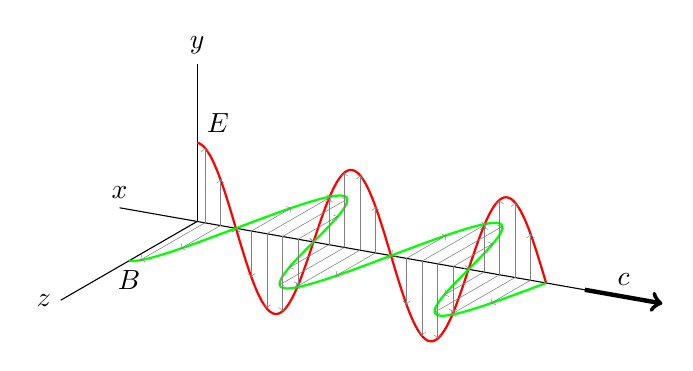
\begin{tikzpicture}[x={(-10:1cm)},y={(90:1cm)},z={(210:1cm)}]
    % Axes
    \draw (-1,0,0) node[above] {$x$} -- (5,0,0);
    \draw (0,0,0) -- (0,2,0) node[above] {$y$};
    \draw (0,0,0) -- (0,0,2) node[left] {$z$};
    % Propagation
    \draw[->,ultra thick] (5,0,0) -- node[above] {$c$} (6,0,0);
    % Waves
    \draw[thick,red] plot[domain=0:4.5,samples=200] (\x,{cos(deg(pi*\x))},0);
    \draw[gray,thick,green] plot[domain=0:4.5,samples=200] (\x,0,{cos(deg(pi*\x))});
    % Arrows
    \foreach \x in {0.1,0.3,...,4.4} {
      \draw[->,help lines] (\x,0,0) -- (\x,{cos(deg(pi*\x))},0);
      \draw[->,help lines] (\x,0,0) -- (\x,0,{cos(deg(pi*\x))});
    }
    % Labels
    \node[above right] at (0,1,0) {$\bm{E}$};
    \node[below] at (0,0,1) {$\bm{B}$};
  \end{tikzpicture}
\end{center}
In questo disegno possiamo vedere le due onde essere perpendicolari fra di loro ed in fase. Esse
inoltre si propagano su un piano perpendicolare a quello di propagazione.\\
Vige anche una proprietà che relaziona i due campi
\begin{equation*}
  c = \frac{E}{B}
\end{equation*}

\subsubsection{Intensità dell'onda}
L'intensità dell'onda (spesso definita anche irradiamento o irraggiamento) è la quantità di energia
che può trasportare l'onda.\\
L'intensità è definita come
\begin{equation*}
  I = \frac{P}{S} = \frac{U}{St}
\end{equation*}
$U$: energia potenziale\\
$S$: superficie\\
$t$: tempo\\ [\baselineskip]
Ma essendo
\begin{equation*}
  U = u\cdot\text{Vol}
\end{equation*}
$u$: densità di energia\\ [\baselineskip]
Quale volume considerare? Possiamo prendere quello che è presente in un periodo
\begin{center}
  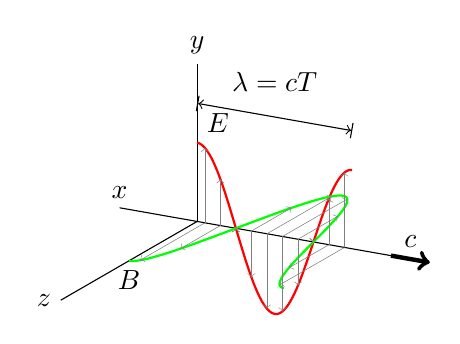
\begin{tikzpicture}[x={(-10:1cm)},y={(90:1cm)},z={(210:1cm)}]
    % Axes
    \draw (-1,0,0) node[above] {$x$} -- (2.5,0,0);
    \draw (0,0,0) -- (0,2,0) node[above] {$y$};
    \draw (0,0,0) -- (0,0,2) node[left] {$z$};
    % Propagation
    \draw[->,ultra thick] (2.5,0,0) -- node[above] {$c$} (3,0,0);
    % Waves
    \draw[thick,red] plot[domain=0:2.0,samples=200] (\x,{cos(deg(pi*\x))},0);
    \draw[gray,thick,green] plot[domain=0:2.0,samples=200] (\x,0,{cos(deg(pi*\x))});
    % Arrows
    \foreach \x in {0.1,0.3,...,1.9} {
      \draw[->,help lines] (\x,0,0) -- (\x,{cos(deg(pi*\x))},0);
      \draw[->,help lines] (\x,0,0) -- (\x,0,{cos(deg(pi*\x))});
    }
    \draw[|<->|] (0,1.5,0) -- ++(2,0,0);
    % Labels
    \node[above right] at (0,1,0) {$\bm{E}$};
    \node[below] at (0,0,1) {$\bm{B}$};
    \node[above] at (1,1.7,0) {$\lambda=cT$};
  \end{tikzpicture}
\end{center}
e quindi il nostro volume diventerebbe, considerando $S$ la superficie su cui stanno i vettori,
\begin{equation*}
  \text{Vol} = ScT
\end{equation*}
e quindi tornando a sostituire
\begin{equation*}
  I = \frac{uScT}{ST} = \bar{u}c
\end{equation*}
Quanto vale $u$ visto che ci sono due campi che variano istante per istante?
\begin{equation*}
  u = u_E + u_B = \frac{1}{2}\varepsilon_0E^2+\frac{1}{2\mu_0}B^2
\end{equation*}
$u_E$: densità di energia del campo elettrico\\
$u_B$: densità di energia del campo magnetico\\ [\baselineskip]
Maxwell aveva anche notato una cosa però
\begin{align*}
  u_E &= \frac{1}{2}\varepsilon_0E^2=\frac{1}{2}\varepsilon_0(cB)^2=\frac{1}{2}c^2B^2=\\
      &= \frac{1}{2}\varepsilon_0 \frac{1}{\varepsilon_0\mu_0}B^2= \frac{1}{2\mu_0}B^2=u_B
\end{align*}
e questo indica che il campo elettrico e il campo magnetico contribuiscono in egual misura
all'intensità dell'onda.\\
Sapendo questo, prima di adattare la formula precedente, dobbiamo trovare un valore medio di $E$
e di conseguenza uno medio di $B$.
\begin{equation*}
  \bar{E^2}=\frac{1}{T}\int_0^T E_0^2\sin^2\alpha\dif\alpha=\frac{E_0^2}{2}
\end{equation*}
E quindi si definisce
\begin{equation*}
  E_{eff} = \frac{E_0}{\sqrt{2}} \qquad B_{eff} = \frac{B_0}{\sqrt{2}}
\end{equation*}
Quindi
\begin{equation*}
  \bar{u}=\frac{1}{2}\varepsilon_0 \frac{E_0^2}{2}+\frac{1}{2\mu_0}\frac{B_0^2}{2}=
  \frac{1}{4}\varepsilon_0E_0^2+\frac{1}{4\mu_0}B_0^2
\end{equation*}
Sostituendo infine
\begin{equation*}
  I=\frac{1}{2}\varepsilon_0E_0^2c=\frac{2}{2\mu_0}B_0^2c=\varepsilon_0E_{eff}^2c=\frac{1}{\mu_0}
  B_{eff}^2c
\end{equation*}

\subsection{Circuiti oscillanti}
I circuiti oscillanti sono dei particolari circuiti LC che generano delle onde elettromagnetiche.
\begin{center}
  \begin{circuitikz}\ctikzset{bipoles/length=.8cm}
    \draw 
    (0,0) 
    to[battery1] (0,1) 
    to[short] (1,1)
    to[C] (1,0)
    to[switch] (1,0)
    to[short] (0,0);
    \draw
    (1,0)
    to[short] (2,0)
    to[L] (2,1)
    to[short] (1,1);
  \end{circuitikz}
\end{center}
Quando il condensatore si carica, l'interruttore non fa arrivare corrente all'induttanza. Alla
chiusura dell'interruttore, il condensatore si scarica attraverso l'induttanza e questo genera
nel condensatore un certo campo elettrico che, per le equazioni di Maxwell, genera un campo
magnetico che propaga l'onda elettromagnetica.\\
Quest'onda avrà una frequenza pari a
\begin{equation*}
  f = \frac{1}{2\pi\sqrt{LC}}
\end{equation*}
Ovviamente perché l'onda venga ricevuta è necessaria un'antenna e un altro circuito oscillante. 
Per ricevere l'onda originale è anche necessario che la frequenza del circuito ricevente sia uguale
a quella del mittente.

\subsection{Equazioni di Maxwell nel mezzo}
Cosa accade alle onde elettromagnetiche che venendo dal vuoto incontrano un mezzo? Definendo
\begin{equation*}
  \varepsilon = \varepsilon_0\varepsilon_r \quad \mu=\mu_0\mu_r
\end{equation*}
Possiamo riscrivere la definizione della velocità
\begin{equation*}
  v = \frac{1}{\sqrt{\varepsilon\mu}} = 
  \frac{1}{\sqrt{\varepsilon_0\mu_0}}\frac{1}{\varepsilon_r\mu_r} =
  \frac{c}{\sqrt{\varepsilon_r\mu_r}}
\end{equation*}
In genere però se un'onda si scontra con un mezzo e quindi viene rifratto. Possiamo quindi 
riprendere le formule dell'ottica
\begin{equation*}
  n = \frac{c}{v}
\end{equation*}
da cui
\begin{equation*}
  v = \frac{c}{n}
\end{equation*}
e quindi
\begin{equation*}
  n = \sqrt{\varepsilon_r\mu_r} 
\end{equation*}
\subsection{Polarizzazione}
Polarizzare un'onda significa ``selezionare'' una parte e bloccarne un'altra.
\subsubsection{Legge di Malus}
I polaroid sono dei filtri polarizzatori, caratterizzati da un'asse di trasmissione.\\
La legge di Malus definisce l'intensità dell'onda dopo il polaroid a seconda se la sorgente
è polarizzata o meno.
\begin{center}
  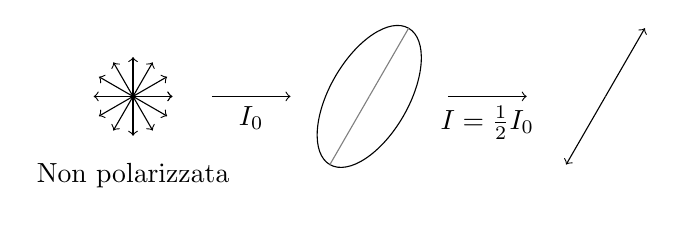
\begin{tikzpicture}
    \foreach \a in {0,30,60,...,360}{
      \draw[->] (0,0) -- (\a:0.5);
    }
    \draw[->] (1,0) -- (2,0)
      node[pos=0.5,below]{$I_0$};
    \filldraw[draw=black,fill=white,rotate around={-30:(3,0)}] (3,0) ellipse (0.5 and 1);
    \draw[thin,gray] (3,0) -- ++(60:1);
    \draw[thin,gray] (3,0) -- ++(240:1);
    \draw[->] (4,0) -- (5,0)
      node[pos=0.5,below]{$I = \frac{1}{2}I_0$};
    \node at (0,-1) {Non polarizzata};
    \draw [->] (6,0) -- ++(60:1);
    \draw [->] (6,0) -- ++(240:1);
  \end{tikzpicture}
\end{center}
Queta vale se la sorgente di luce non è polarizzata, quindi una lampadina ad esempio.
\begin{center}
  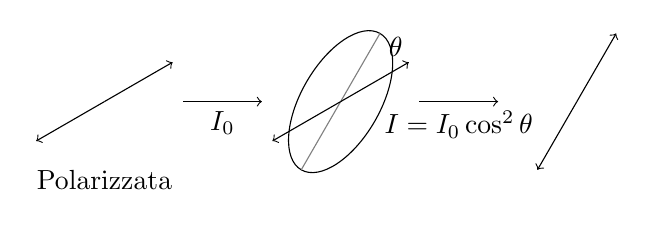
\begin{tikzpicture}
    \draw[->](0,0) -- ++(30:1);
    \draw[->] (0,0) -- ++(210:1);
    \draw[->] (1,0) -- (2,0)
      node[pos=0.5,below]{$I_0$};
    \filldraw[draw=black,fill=white,rotate around={-30:(3,0)}] (3,0) ellipse (0.5 and 1);
    \draw[thin,gray](3,0) -- coordinate(A) ++(60:1);
    \draw[thin,gray] (3,0) -- ++(240:1);
    \draw[->](3,0) -- coordinate (B) ++(30:1);
    \draw[->] (3,0) -- ++(210:1);
    %\coordinate (A) at (3,0)+(30:1);
    \coordinate (O) at (3,0);
    %\coordinate (B) at (3,0)+(60,1);
    \markangle{A}{O}{B}{0.6}{1.2}{$\text{ }$}
    \node at (3.7,0.7) {$\theta$};
    \draw[->] (4,0) -- (5,0)
      node[pos=0.5,below]{$I = I_0\cos^2\theta$};
    \node at (0,-1) {Polarizzata};
    \draw[->] (6,0) -- ++(60:1);
    \draw[->] (6,0) -- ++(240:1);
  \end{tikzpicture}
\end{center}
$\theta$: angolo tra l'asse di trasmissione e quello della luce polarizzata

\subsubsection{Angolo di Brewster}
Ogni raggio riflesso e rifratto è parzialmente polarizzato. L'angolo di Brewster è quel particolare
angolo in cui la polarizzazione è massima ed è rappresentato dal seguente disegno.
\begin{center}
  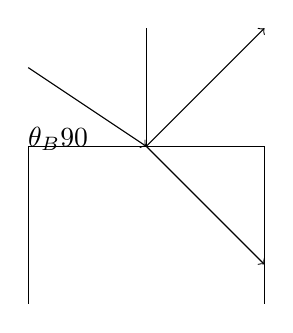
\begin{tikzpicture}
    \draw (0,-2) -- (0,0) -- ++(3,0) -- ++(0,-2);
    \coordinate (In) at (0,1);
    \coordinate (Center) at (1.5,0);
    \coordinate (OutB) at (3,1.5);
    \coordinate (OutR) at (3,-1.5);
    \coordinate (OutM) at (1.5,1.5);
    \draw[->] (In) -- (Center);
    \draw[->] (Center) -- (OutB);
    \draw[->] (Center) -- (OutR);
    \draw (Center) -- (OutM);
    \markangle[cyan]{Center}{In}{OutM}{1}{1.5}{$\theta_B$}
    \markangle[orange]{Center}{OutB}{OutR}{1}{1.5}{$\ang{90}$}
  \end{tikzpicture}
\end{center}
Dato che gli indici di rifrazione sono diversi, possiamo scrivere per la relazione di Snell
\begin{equation*}
  n_1\sin\theta_B = n_2\sin\hat{r}
\end{equation*}
e vedendo che $\hat{r} = 90-\theta_B$ e quindi
\begin{equation*}
  n_1\sin\theta_B = n_2\sin(90-\theta_B) = \cos\theta_B
\end{equation*}
E quindi
\begin{equation*}
  \theta_B = \arctan\frac{n_2}{n_1}
\end{equation*}
